\documentclass{article}
\usepackage{fullpage}
\usepackage{graphicx}
\usepackage{minted}
\usepackage{booktabs}
\usepackage{hyperref}
\usepackage[margin=1.5cm, includefoot, footskip=30pt]{geometry}

\title{The Mann Whitney U Test \\ \large Investigating Homelessness Rates in England}
\author{Geraint Palmer - C1016865}
\date{}

\begin{document}

\maketitle

\section{The Problem}
In this report homeless rates are investigated for the local authorities of
England.
In particular differences in the homeless rates of the north and south of the
country, as well as London, are looked at.
The statstic we will look at is the number of people presumed homeless per 1000
residents, for each local authority.

The government releases publically available data on homelessness \cite{data},
and for this work a sample of 30 local authorities from the north of England, 30
from the south, and 30 from London are taken; a sample is shown in the table
below.

\begin{table}[h]
\centering
\footnotesize{
\begin{tabular}{lllr}
\toprule
         Local Authority &  Region &  Homeless per 1000 \\
\midrule
              Rossendale &   South &               0.46 \\
              Calderdale &   South &               0.22 \\
                   Brent &  London &               0.64 \\
  Kensington and Chelsea &  London &               1.12 \\
                  Thanet &   North &               0.71 \\
                 Lambeth &  London &               0.53 \\
\bottomrule
\end{tabular}
}
\end{table}

Parametric tests can compare mean homeless rates between the regions, if the
rates are Normally distributed.
Using \texttt{matplotlib}, the following histograms show that they are not.
So another method will be required.

\begin{figure}[h]
\centering
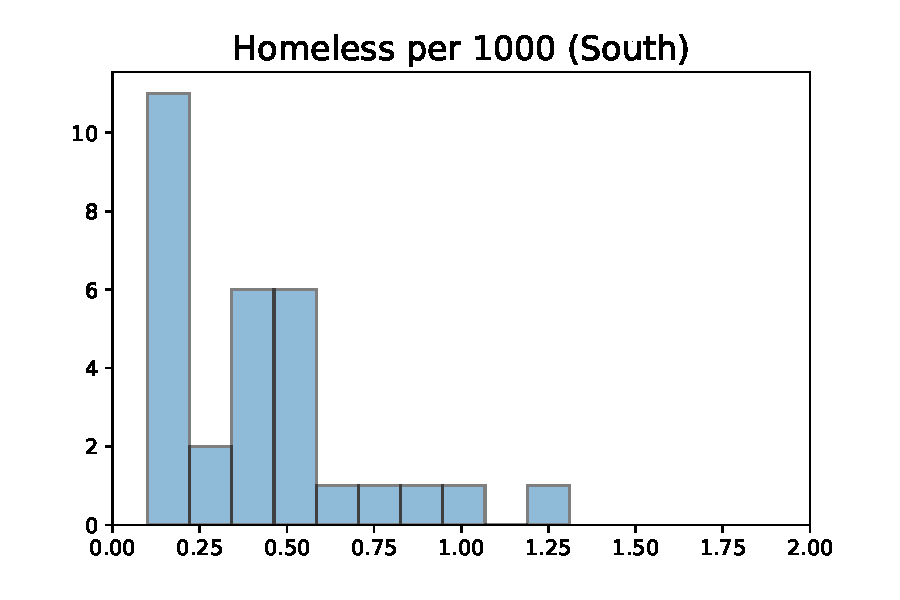
\includegraphics[width=0.3\textwidth]{south_homeless.pdf}
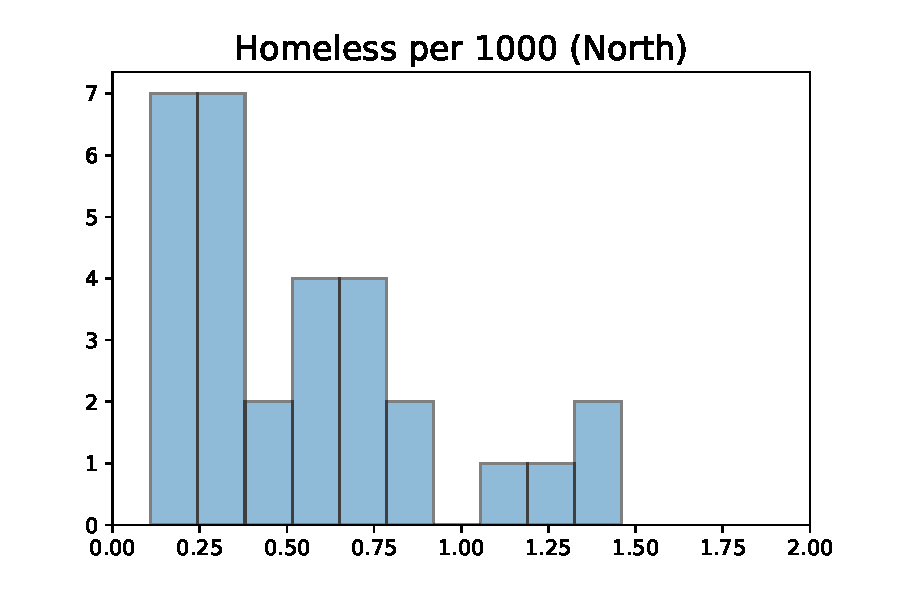
\includegraphics[width=0.3\textwidth]{north_homeless.pdf}
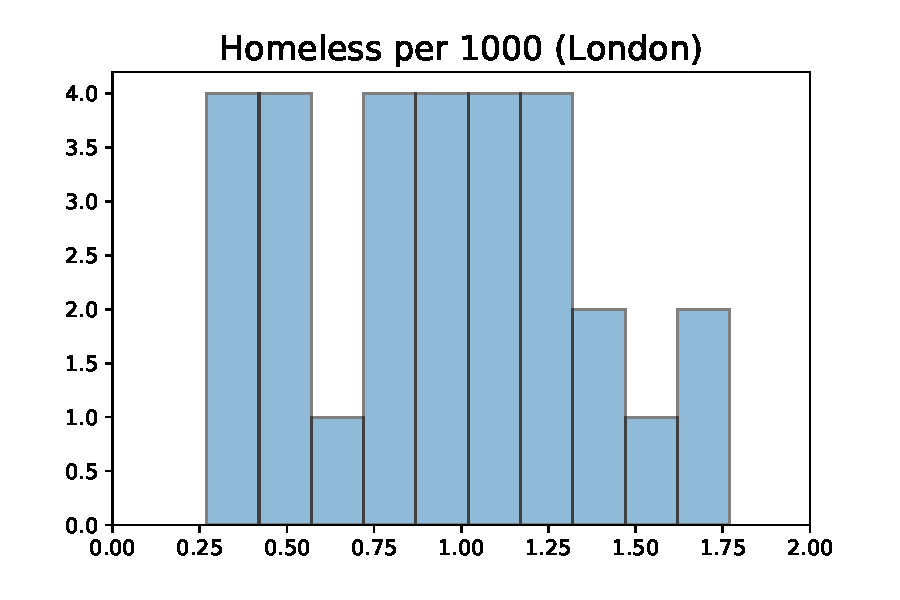
\includegraphics[width=0.3\textwidth]{london_homeless.pdf}
\end{figure}

\section{Solution Method}
In order to compare centrality measures for data that is not Normally
distributed, non-parametric tests are required.
Here the Mann-Whitney U test will be used \cite{mannwhitneyu}, which compares
medians of two independent samples.

In order to conduct the test, on two independent samples of sizes $n_1$ and
$n_2$, the following steps are to be undertaken:

\begin{enumerate}
  \setlength\itemsep{0em}
  \item Sort the two independent samples.
  \item Convert the sample values to overall ranks.
  \item Obtain $R_1$ and $R_2$, the sums of the ranks of each sample.
  \item Obtain $U_1 = R_1 - \left(\frac{1}{2} n_1 (n_1 + 1)\right)$ and $U_2 = R_2 - \left(\frac{1}{2} n_2 (n_2 + 1)\right)$.
  \item Obtain the $U = \min(U_1, U_2)$.
  \item Use a standard Normal approximation $z = \frac{U - \mu}{\sigma}$, where $\mu = \frac{1}{2} n_1 n_2$ and $\sigma = \sqrt{\frac{1}{12} n_1 n_2 (n_1 + n_2 + 1)}$.
  \item Find the p-value $P(Z \leq z)$, where $Z \sim N(0, 1)$.
\end{enumerate}

This algorithm is coded as a function \texttt{mann\_whitney\_u}, which takes two
lists of values as inputs, and outputs a p-value.
This function is attached as an appendix.
Most of the steps can be implemented with standard Python arithmetic and
methods.
Step 7 requires the library \texttt{scipy} in order to get percentage points of
the standard Normal distribution.
Step 2 is also more involved, and requires looping though the ranks using a
while loop, identifying which sample the next ranking observation comes from,
then appending the current rank to the list.

\section{Code Use \& Discussion}

A Mann-Whitney test is conducted, with $\alpha=0.05$, testing whether there is
a difference in homeless rates of the north and south of England:

\begin{itemize}
  \setlength\itemsep{-0.5em}
  \item $H_0$: The median homeless rate of the south is equal to the median
  homeless rate of the north.
  \item $H_1$: The median homeless rate of the south is lower than the median
  homeless rate of the north.
\end{itemize}

\begin{minted}{python}
>>> mann_whitney_u(data_south, data_north)
0.0620756405457464
\end{minted}

A p-value of 0.062 is obtained, and so the null hypothesis cannot be rejected.

Another test is conducted, with $\alpha = 0.05$, testing whether there is a
difference in the homeless rates of London compared to the rest of England:

\begin{itemize}
  \setlength\itemsep{-0.5em}
  \item $H_0$: The median homeless rate of London is equal to the median
  homeless rate of the rest of England.
  \item $H_1$: The median homeless rate of London is higher than the median
  homeless rate of the rest of England.
\end{itemize}

\begin{minted}{python}
>>> mann_whitney_u(data_north+data_south, data_london)
4.388061912191502e-07
\end{minted}

A p-value of 0.00000004388 is obtained, and so the null hypothesis is rejected,
and we conclude that London has a higher median homeless rate than the rest of
England.

\begin{thebibliography}{9}

\bibitem{data}
  Ministry of Housing, Communities \& Local Government,
  Live tables on homelessness,
  \url{https://www.gov.uk/government/statistical-data-sets/live-tables-on-homelessness},
  2018.

\bibitem{mannwhitneyu}
   Wackerly, Dennis, William Mendenhall, and Richard L. Scheaffer.
   Mathematical statistics with applications.
   Cengage Learning,
   2014.

\end{thebibliography}

\newpage

\small{
\begin{minted}{python}
def mann_whitney_u(data1, data2):
    # Get sorted data
    data1 = sorted(data1)
    data2 = sorted(data2)
    
    # Get numbers of observations
    n1 = len(data1)
    n2 = len(data2)
    max_rank = len(data1) + len(data2)
    
    # Placeholders to keep the ranks
    ranks1 = []
    ranks2 = []
    current_rank = 1
    
    # Place rank in correct holder
    while current_rank <= max_rank:
        if len(data2) == 0:
            ranks1.append(current_rank)
            current_rank += 1
            data1.pop(0)
        elif len(data1) == 0:
            ranks2.append(current_rank)
            current_rank += 1
            data2.pop(0)
        else:
            if data1[0] == data2[0]:
                ranks1.append(current_rank + 0.5)
                ranks2.append(current_rank + 0.5)
                current_rank += 2
                data1.pop(0)
                data2.pop(0)
            elif data1[0] < data2[0]:
                ranks1.append(current_rank)
                current_rank += 1
                data1.pop(0)
            elif data2[0] < data1[0]:
                ranks2.append(current_rank)
                current_rank += 1
                data2.pop(0)
    
    # Get rank sums and U statistic
    R1 = sum(ranks1)
    R2 = sum(ranks2)
    U1 = R1 - ((n1 * (n1 + 1)) / 2)
    U2 = R2 - ((n2 * (n2 + 1)) / 2)
    U = min(U1, U2)
    
    # Normal approximation
    mu = (n1 * n2) / 2
    sg = ((n1 * n2 * (n1 + n2 + 1)) / 12) ** 0.5
    z = (U - mu) / sg
    p_val = scipy.stats.norm(0, 1).cdf(z)
    return p_val
\end{minted}
}

\end{document}